\documentclass[10pt, sans, compress, usenames, dvipsnames, aspectratio=169]{beamer}

%% Import the template configuration
\usepackage[T1]{fontenc}
\usepackage{lmodern}
\usepackage{graphicx}
\usepackage[french]{babel}
\usepackage[utf8]{inputenc}
\usetheme{Warsaw}
\usepackage{wasysym}
\usepackage{tabularx}
\usepackage{hyperref}
\usepackage[absolute,overlay]{textpos}
\setbeamertemplate{navigation symbols}{}
\useoutertheme{infolines}
\useinnertheme{rectangles}
\setbeamertemplate{background canvas}{
\includegraphics[width=\paperwidth,height=\paperheight]{images/ucabackground-16_9.png}}
\usepackage{caption}
\captionsetup{figurename=}
\definecolor{uca01}{HTML}{006E83}
\definecolor{uca02}{HTML}{0096A0}
\definecolor{uca03}{HTML}{006C82}
\definecolor{uca04}{HTML}{0398A1}
\definecolor{uca05}{HTML}{585656}
\definecolor{uca06}{HTML}{438D97}
\definecolor{grisuca}{HTML}{5E5C5C}


\setbeamercolor{palette primary}{bg=uca06}
\setbeamercolor{palette secondary}{bg=uca03}
\setbeamercolor{palette tertiary}{bg=uca04}
\setbeamercolor{palette quaternary}{bg=uca05}
\setbeamercolor{block title}{bg=uca06}
\setbeamercolor{itemize item}{fg=uca03}
\setbeamercolor{itemize subitem}{fg=uca03}
\setbeamercolor{itemize subsubitem}{fg=uca03}


\setbeamercolor{enumerate item}{bg=uca03,fg=uca03}
\setbeamercolor{enumerate subitem}{bg=uca03,fg=uca03}
\setbeamercolor{enumerate subsubitem}{bg=uca03,fg=uca03}
\setbeamercolor{enumerate mini template}{bg=uca03,fg=uca03}
\setbeamercolor{itemize body}{fg=uca03}
\setbeamercolor{itemize subbody}{fg=uca03}
\setbeamercolor{itemize subsubbody}{fg=uca03}
\setbeamercolor{enumerate body}{fg=uca03}
\setbeamercolor{enumerate subbody}{fg=uca03}
\setbeamercolor{enumerate subsubbody}{fg=uca03}

\setbeamercolor{item projected}{bg=uca03}
\setbeamercolor{section in toc}{fg=grisuca}
\setbeamercolor{normal text}{fg=grisuca}



\title{Reproducibility: an old friend, the laboratory notebook}
\subtitle{Better reproducibility with documented code \footnote{This work is derived from the IFB and I2BC team members}}

\author[Pierre MARIN]{Pierre Marin\\\texttt{pierre.marin@uca.fr}}
\institute{Université Clermont Auvergne, AuBi, Mésocentre}
\date{\today}

\newif\iflattersubsect

% \AtBeginSubsection[] {
%     \iflattersubsect
%     \begin{frame}<beamer>
%     \frametitle{Sommaire} %
%     \tableofcontents[currentsubsection]
%     \end{frame}
%     \fi
%     \lattersubsecttrue
% }

\begin{document}
% titre et sommaire

\begin{frame}
  \titlepage
  \begin{textblock*}{5cm}(2cm,0.5cm) % {block width} (coords)
  
\includegraphics[width=2.3cm,height=1.3cm]{images/logo_ifb.pdf}
  \end{textblock*}
  \begin{textblock*}{5cm}(13cm,0.3cm) % {block width} (coords)
  
\includegraphics[width=1.5cm,height=1.5cm]{images/i2bc.png}
  \end{textblock*}
  \begin{textblock*}{5cm}(2cm,4cm) % {block width} (coords)
  
\includegraphics[width=3.5cm,height=3cm]{images/logoAuBi-2019.pdf}
  \end{textblock*}
  \begin{textblock*}{5cm}(12cm,3.6cm) % {block width} (coords)
  
\includegraphics[width=3cm,height=3cm]{images/mesocentre.png}
  \end{textblock*}
   \begin{textblock*}{5cm}(12.5cm,6cm) % {block width} (coords)
  
\includegraphics[width=2cm,height=1.5cm]{images/medis_logo.png}
  \end{textblock*}
\end{frame}
\begin{frame}
  \frametitle{Sommaire}
   \tableofcontents
\end{frame}

% cahier de manip
\section{The laboratory notebook}
\subsection{The aim}
\begin{frame}[<+->]{Paper version}
\begin{textblock*}{10cm}(1cm,2cm) % {block width} (coords)
Laboratory notebook allow to:
\begin{itemize}
	\item Day-to-day recording each step in a process, experiments...
	\item Report on the progress, and scientific experimentations \newline
	from the idea to final conclusions
	\item Keep track of knowledge in a lab
	\item Useful drafting a patent
	\item Proof of anteriority
\end{itemize}
\end{textblock*}
\only<1>{
\begin{textblock*}{10cm}(1cm,3cm) % {block width} (coords)
  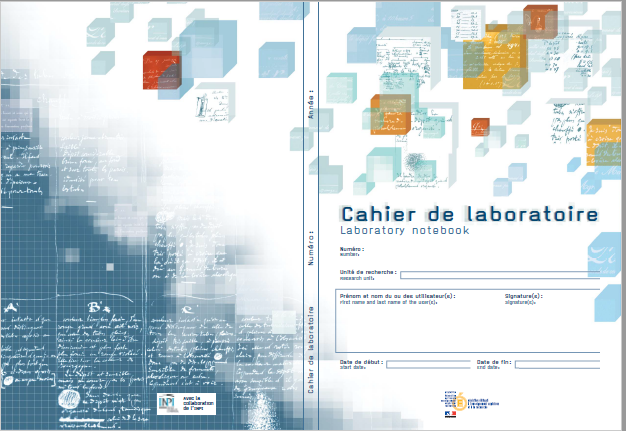
\includegraphics[width=7cm,height=5cm]{images/cahierlabo.png}
 \end{textblock*}
 \begin{textblock*}{10cm}(8cm,3cm) % {block width} (coords)
  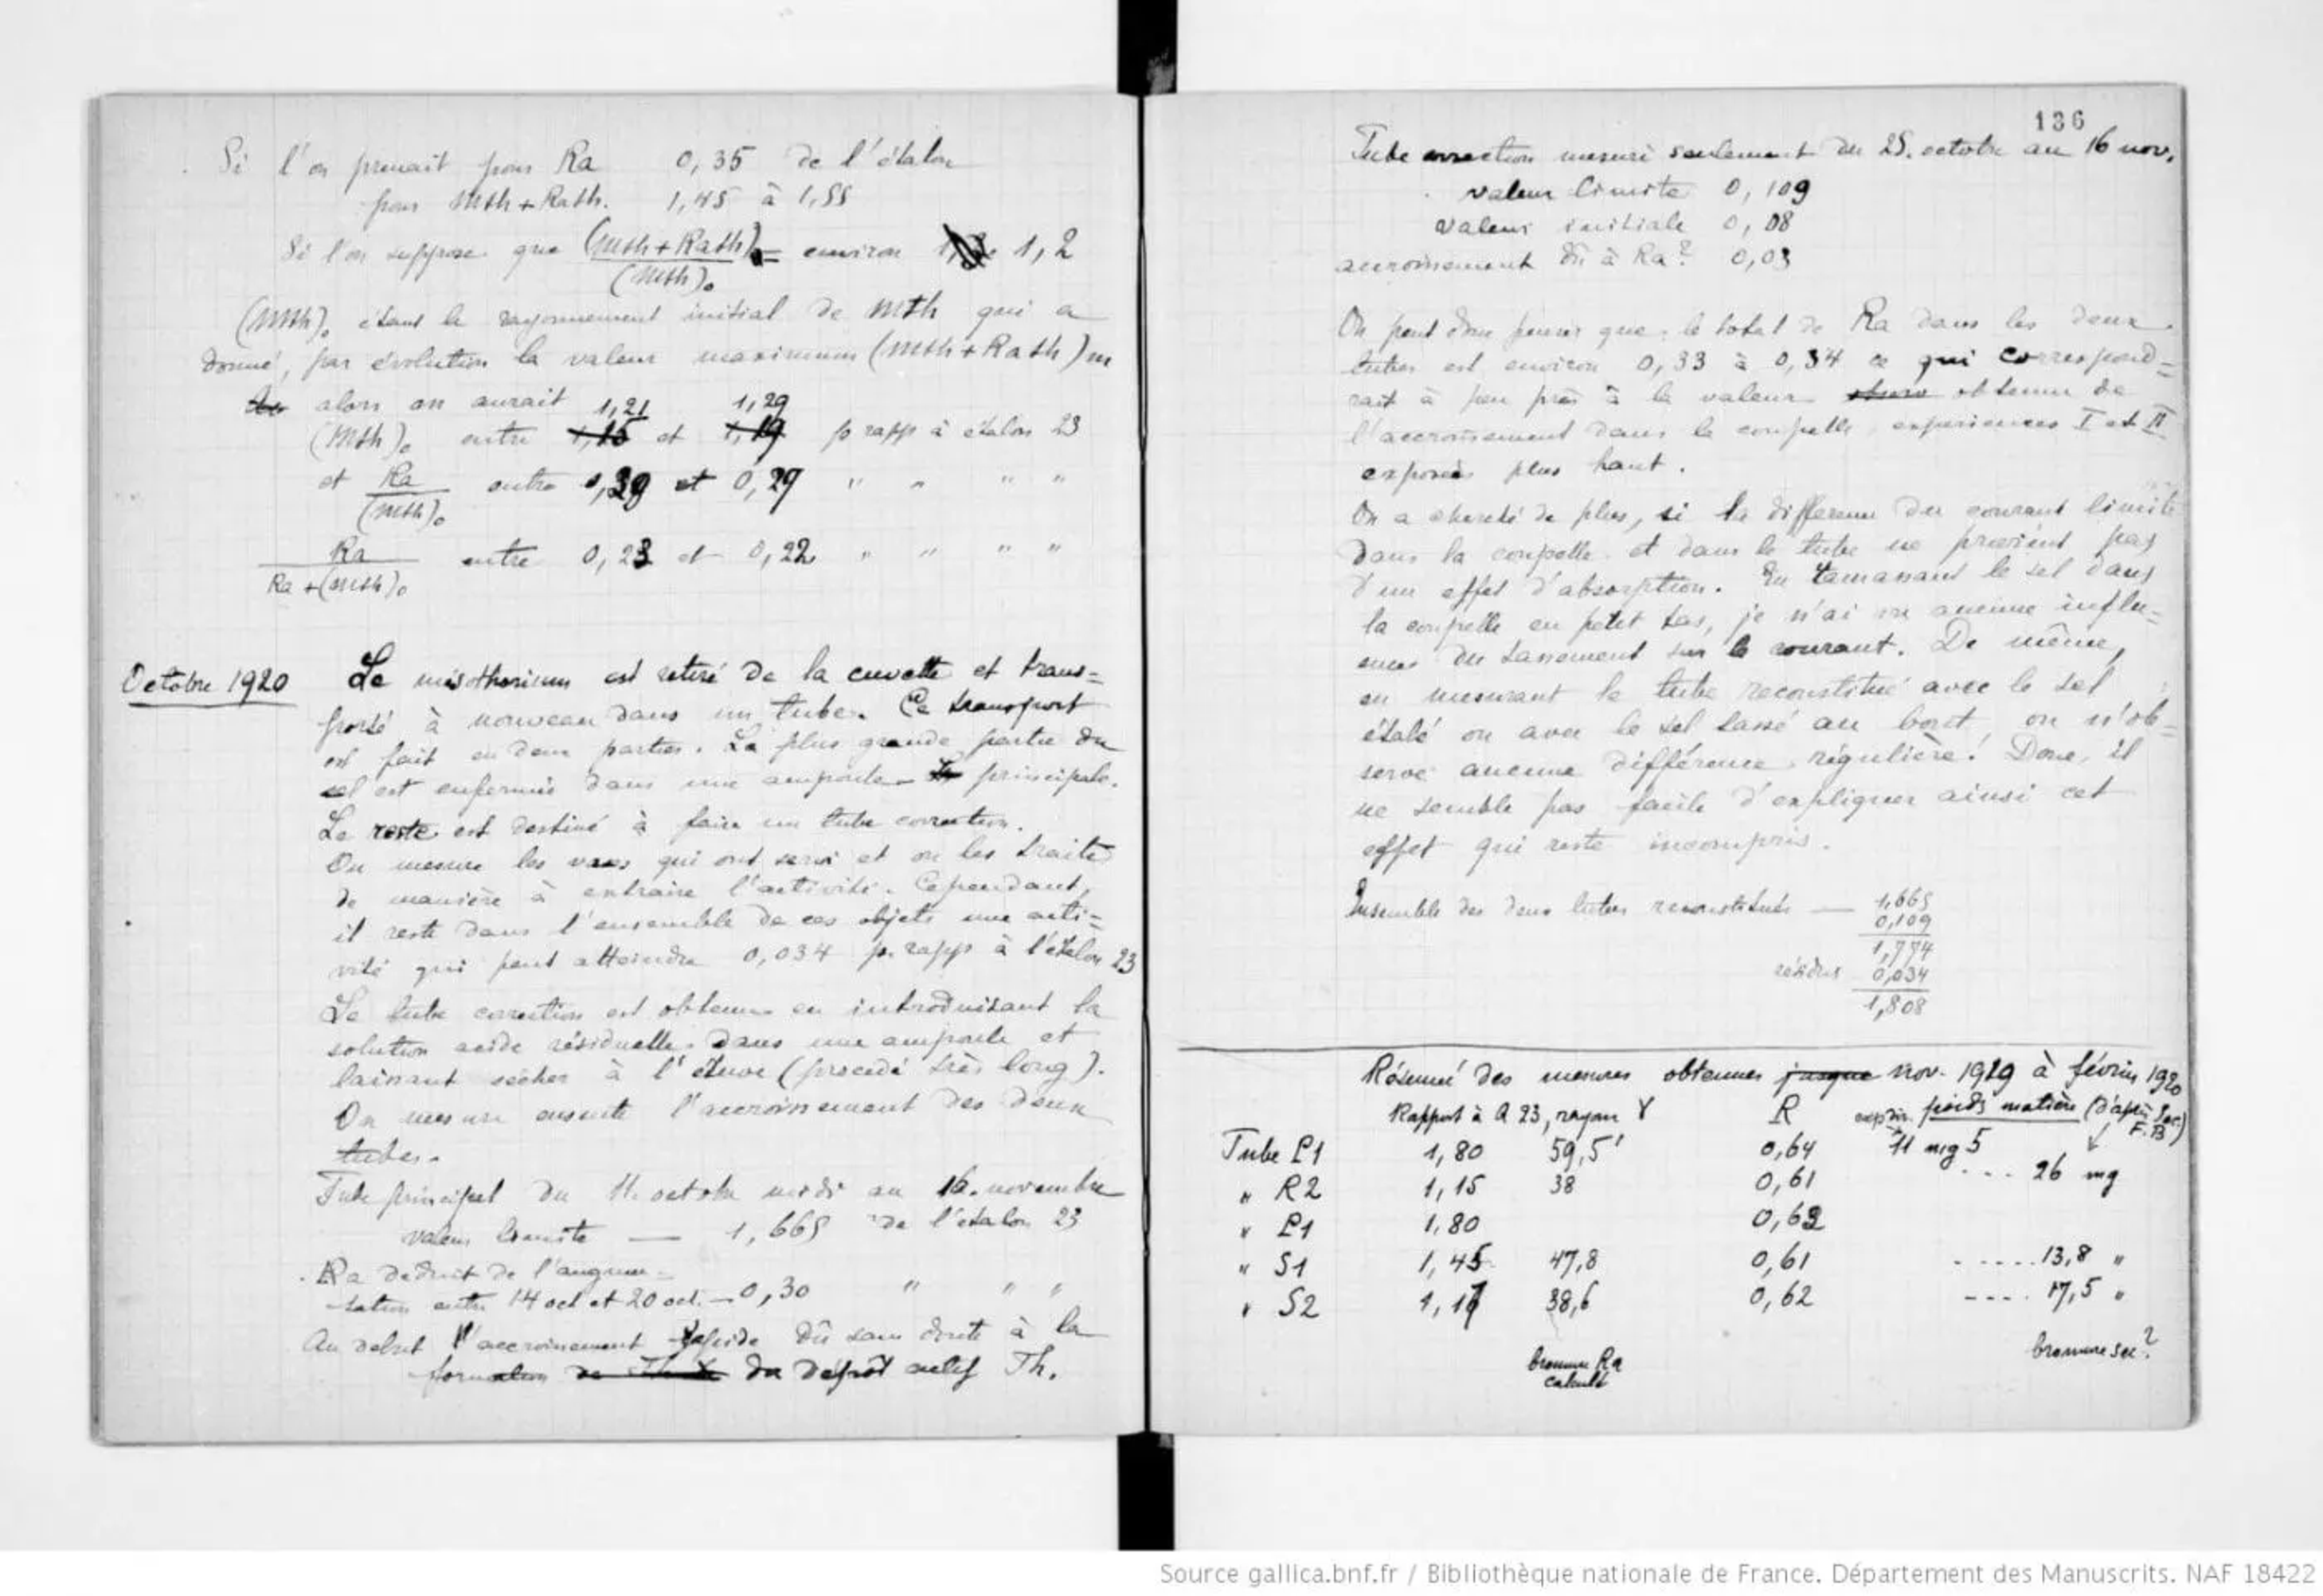
\includegraphics[width=7cm,height=5cm]{images/cahier2.pdf}
 \end{textblock*}}
\end{frame}

\begin{frame}[<+->]{Paper version}
\begin{columns}
\column{.5\textwidth}
This is a legal tool:
 \begin{itemize}
 \item Page numbered in each notebook
 \item Cover page with the owner of the results
 \item Each page contain a part to date, to sign for at least to people
 \end{itemize}
\column{.5\textwidth}
At each research level:
  \begin{itemize}
 \item Researchers
 \item Engineers
 \item Technicians
 \item Students...
 \end{itemize}
\end{columns}
\vspace{1cm}
\onslide<10>{\centering End what's happen for bioinformatic ?}
\end{frame}

\begin{frame}[<+->]{Electronic version}
\onslide<1->{Electronic Laboratory Notebooks (ELN)} \newline
\onslide<1->{Modern LN since 2009 (C.U.R.I.E. Network)}
\only<2>{
\begin{textblock*}{10cm}(9cm,2cm) % {block width} (coords)

\includegraphics[width=3cm,height=1cm]{images/elabftw-logo.png}
\end{textblock*}
\begin{textblock*}{10cm}(0.5cm,4cm) % {block width} (coords)
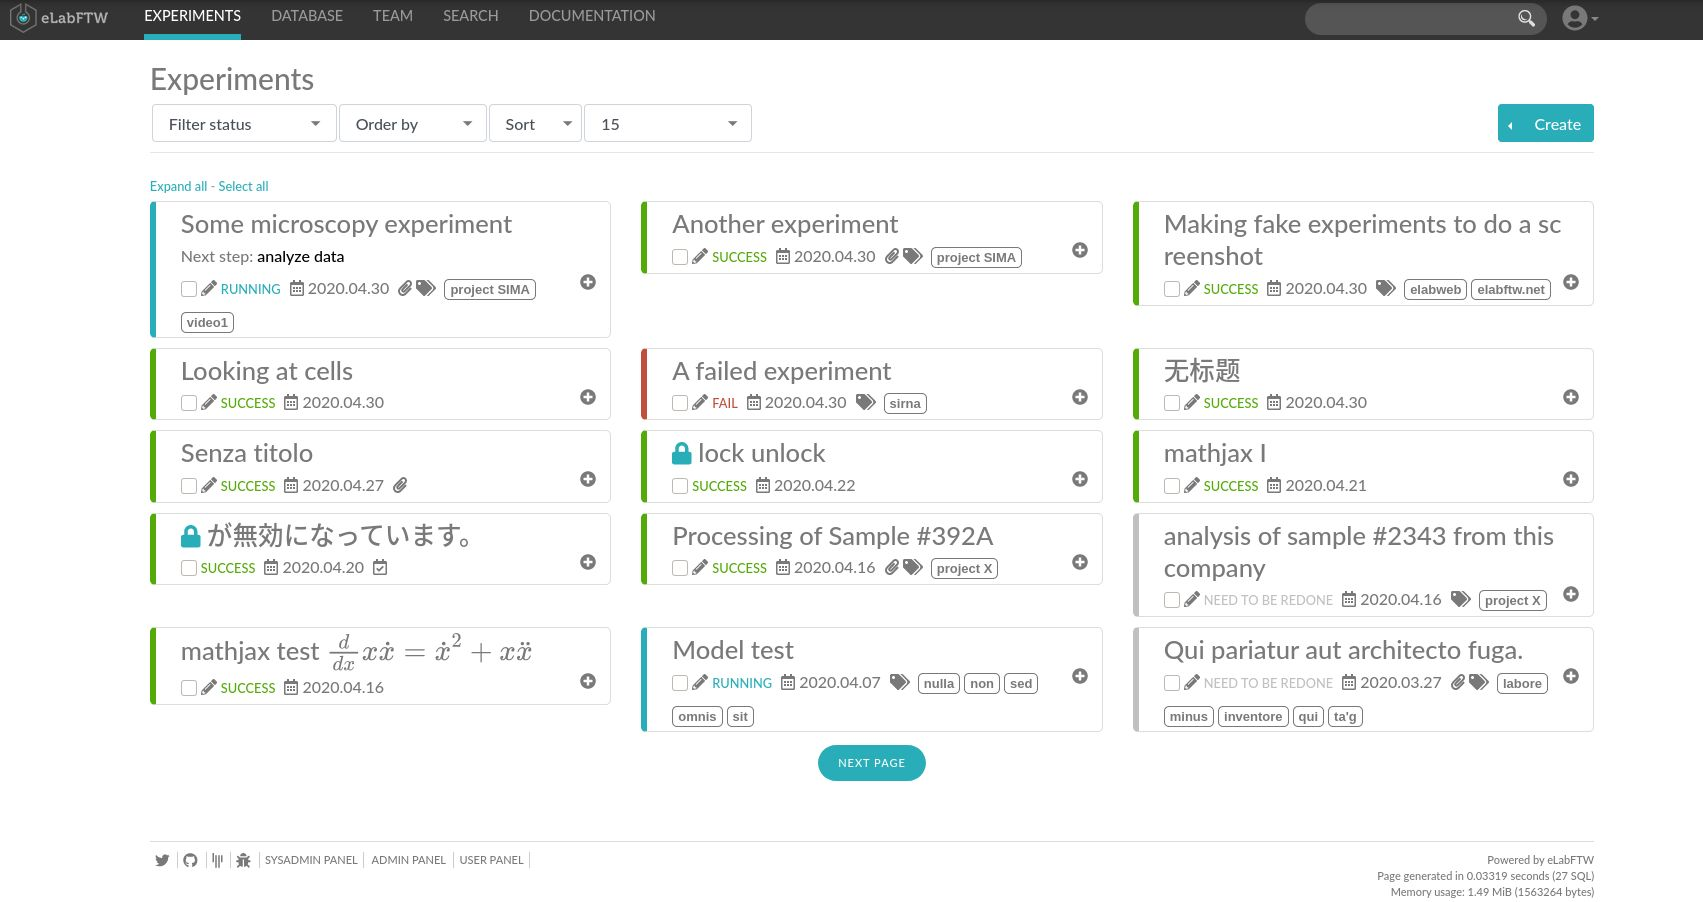
\includegraphics[width=7cm,height=4cm]{images/elabftw1.jpg}
\end{textblock*}
\begin{textblock*}{10cm}(8cm,4cm) % {block width} (coords)
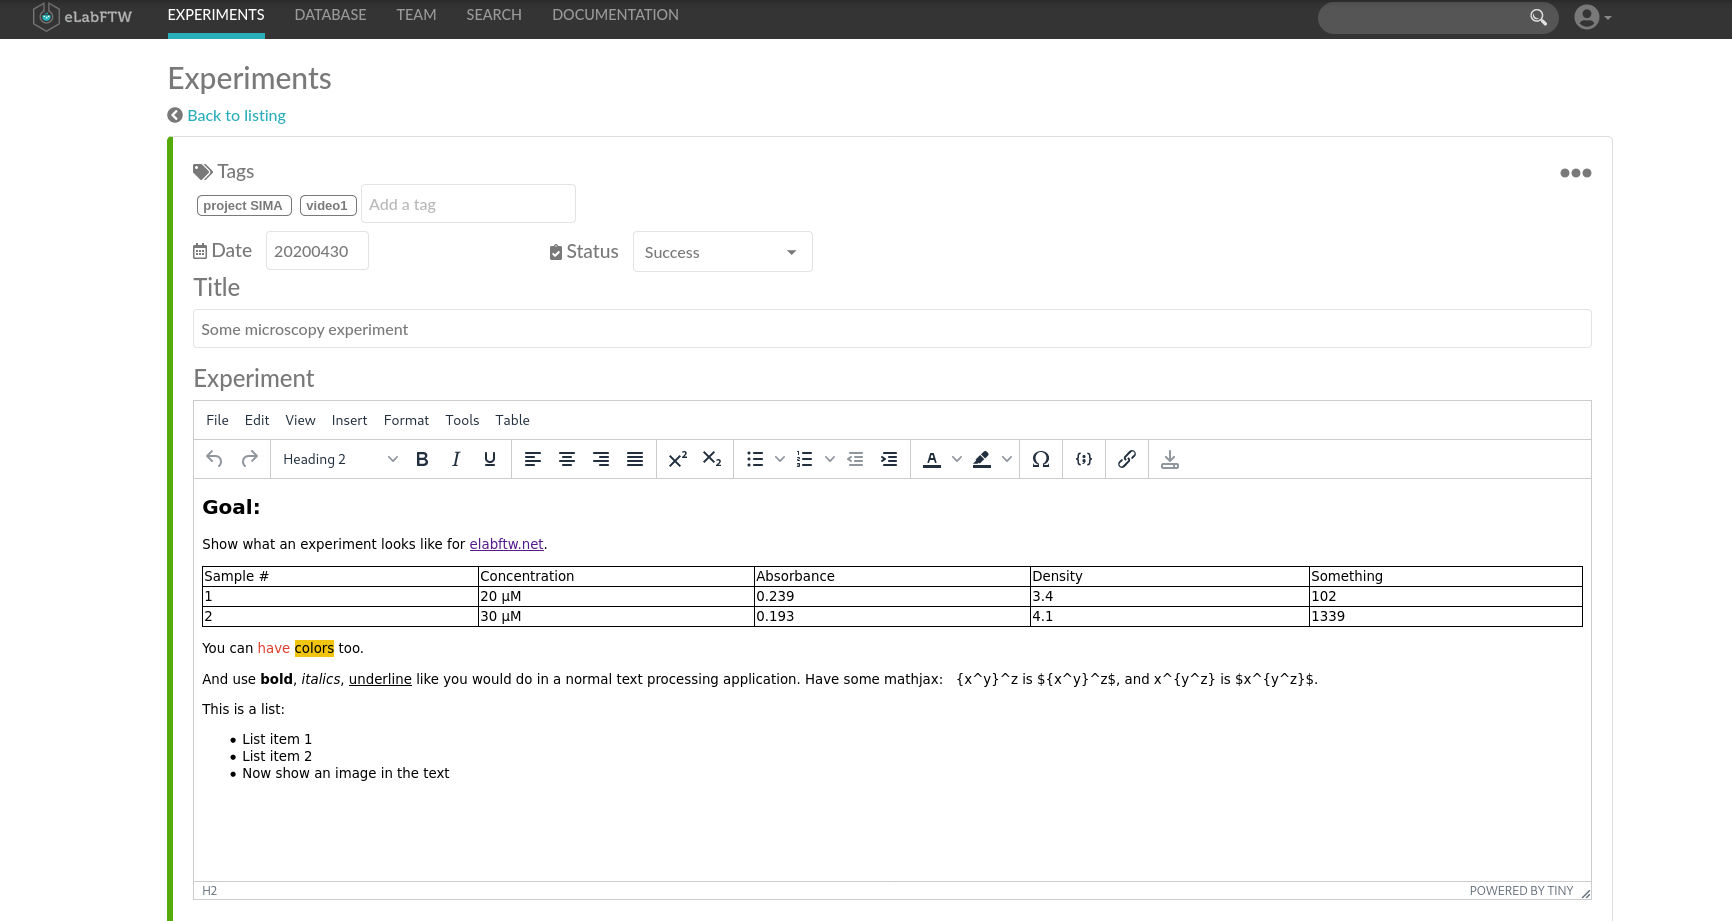
\includegraphics[width=7cm,height=4cm]{images/elabftw2.jpg}
\end{textblock*}}
\onslide<3->{
 \begin{itemize}
 	\item dematerialised
 	\item archivable
 	\item sharable
 	\item secure
 \end{itemize}}
\onslide<4->{
\centering But less and less adapted to recent evolutions of our work \\
\centering We need an electronic tool for individual traceability}
\end{frame}

\begin{frame}{Electronic version}
\only<1>{\centering
\includegraphics[width=10cm,height=7cm]{images/gt_eln.png}}
\only<2>{\centering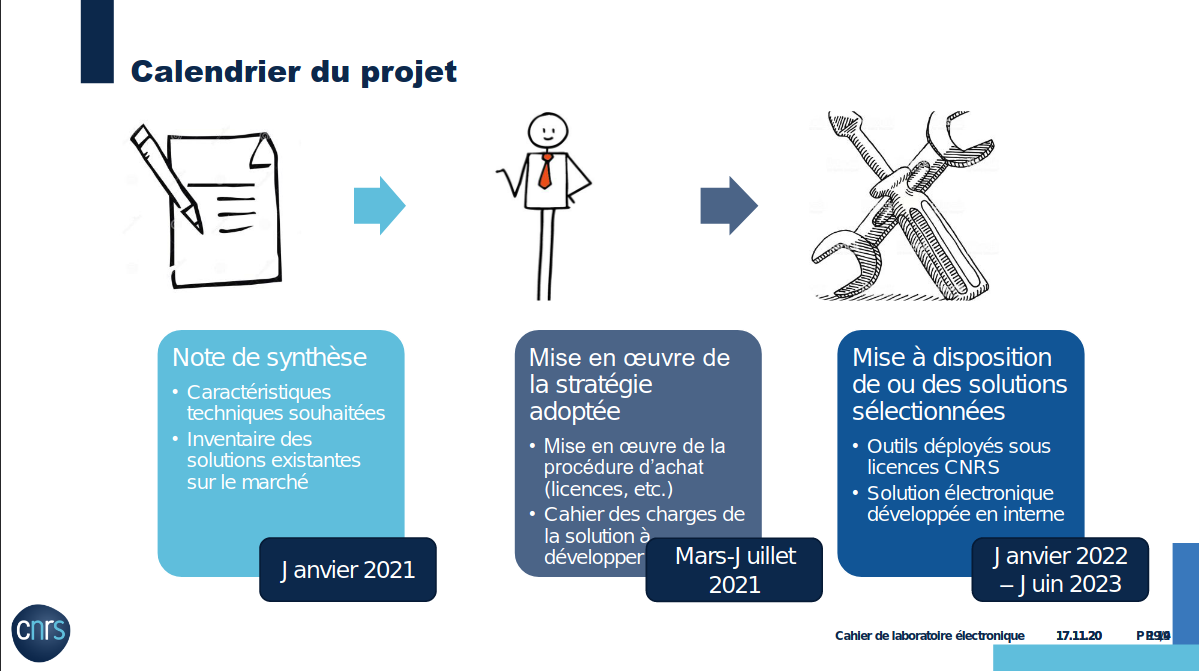
\includegraphics[width=10cm,height=7cm]{images/gt_eln_temp.png}}
\end{frame}


% les notebook
\section{Notebook in bioinformatic}
\subsection*{Literate programming}
\begin{frame}{Literate programming}
\onslide<1->{What is literate programming ?}\newline
\onslide<2->{\emph{
"Let us change our traditional attitude to the construction of programs: \\
Instead of imagining that our main task is to instruct a computer what to do, let us concentrate rather on explaining to humans what we want the computer to do."}
\footnote{Donald E. Knuth, Literate Programming, 1984} }
\newline
\vspace{1cm}
\onslide<3->{\emph{
”Literate programming is a programming paradigm introduced by Donald Knuth in
which a computer program is given an explanation of its logic in a natural language,
such as English, interspersed with snippets of macros and traditional source code,
from which compilable source code can be generated.”}
\footnote{\url{https://en.wikipedia.org/wiki/Literate_programming\# Workflow}}
}
\end{frame}

\begin{frame}{Literate programming}
\onslide<1,3->{What does it look like ?}\newline
\onslide<3->{Interactive programming interface allowing to combine both natural and computer languages \\}
\onslide<4->{In one file}
\begin{itemize}[<4->]
	\item Explanation
	\item Code
	\item Results
	\item Graphs and plots
\end{itemize}
\begin{textblock*}{5cm}(3cm,2cm) % {block width} (coords)
\only<2>{\centering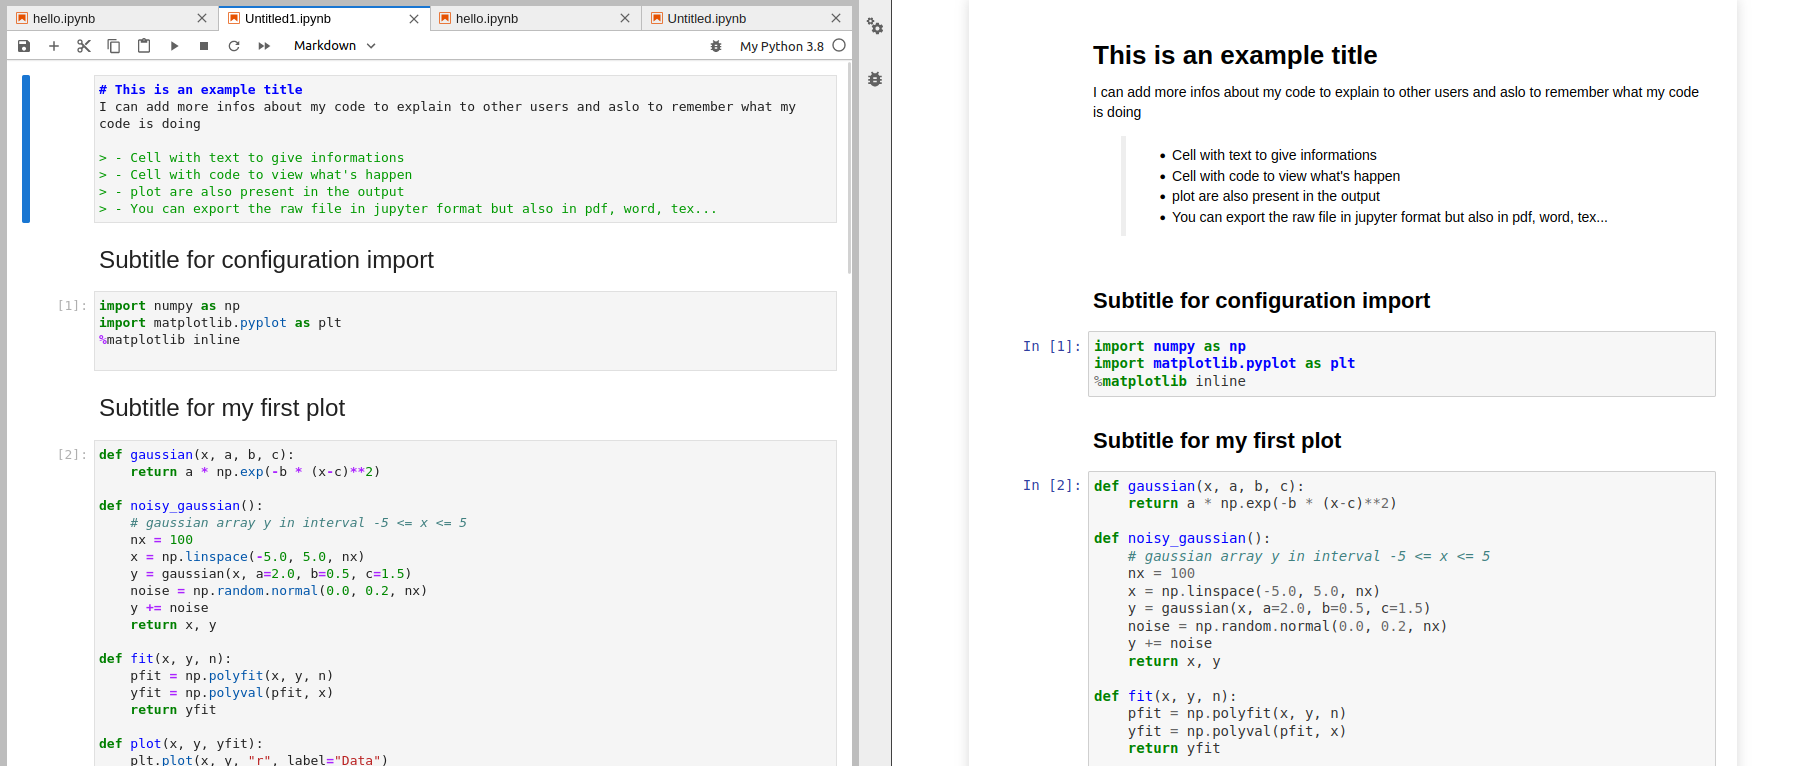
\includegraphics[width=12cm,height=6cm]{images/jupyter_example.png}}
\end{textblock*}
\end{frame}

\begin{frame}{Literate programming}
Why using literate programming frameworks ?
\begin{itemize}[<+->]
	\item Labbook
	\item Day-to-day analysis
	\item Make automatic reports
	\item Write scientific article
\end{itemize}
\end{frame}

\begin{frame}{Literate programming}{example}
\onslide<1>{Example of an article written using a notebook
\footnote{\url{https://www.frontiersin.org/articles/10.3389/fphys.2018.00787/full}}}
\only<2>{
\begin{figure}
\centering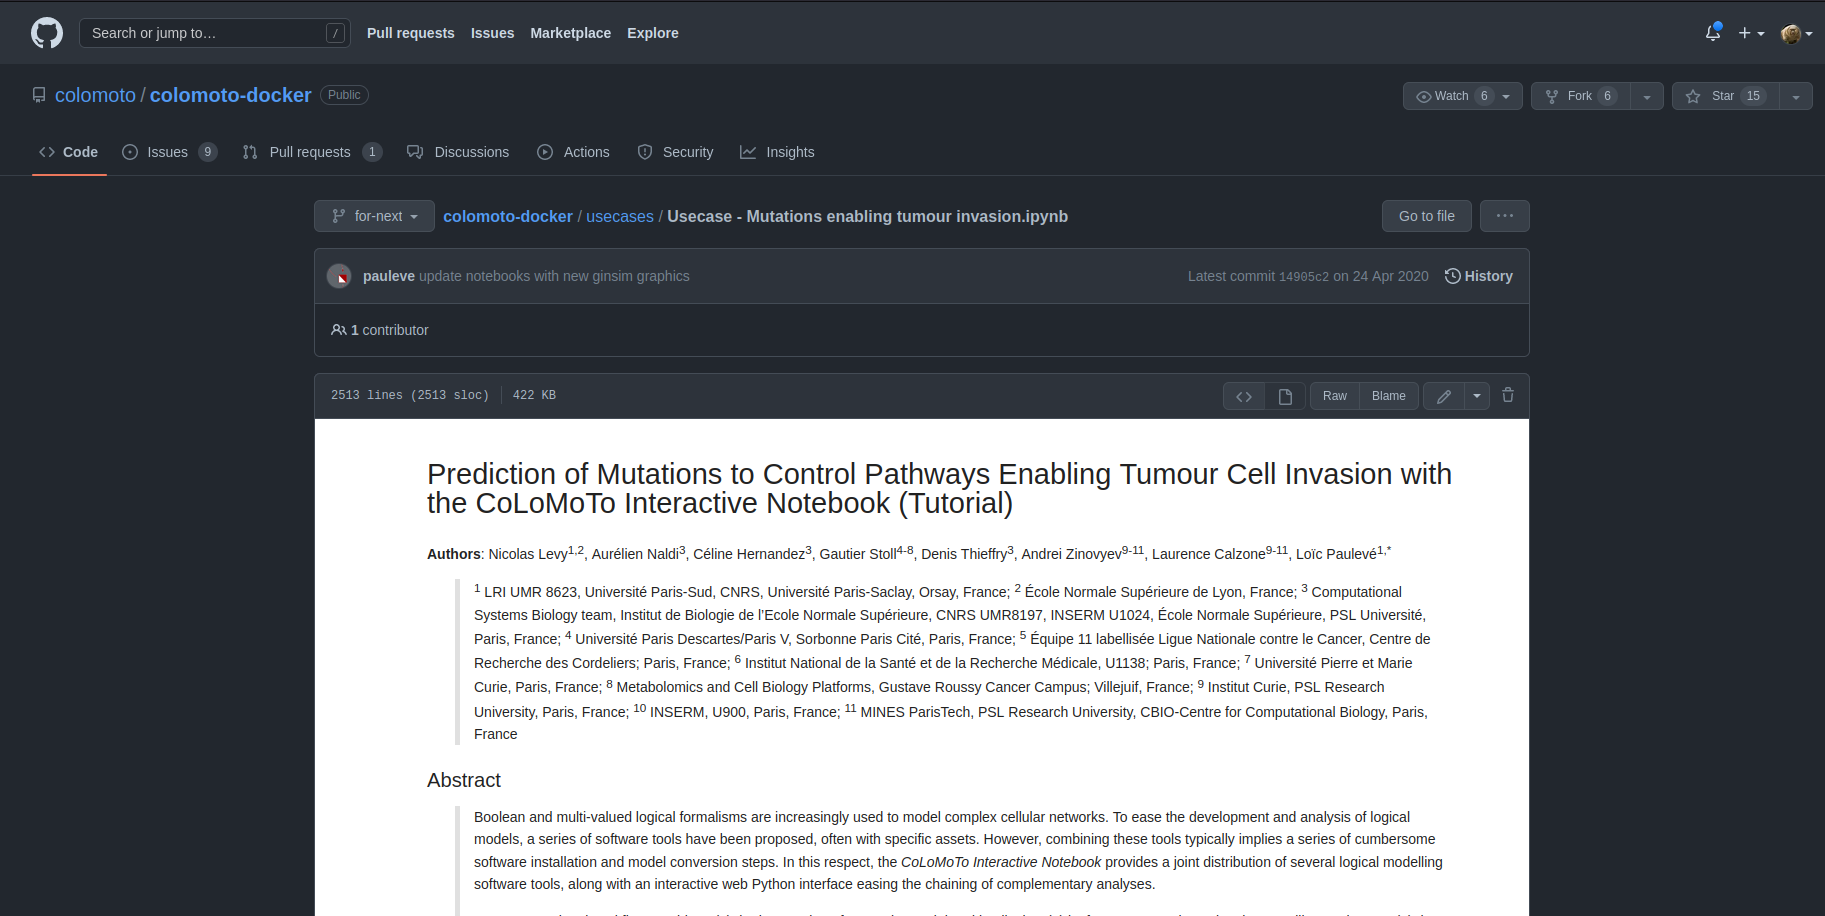
\includegraphics[width=15cm,height=9cm]{images/colomoto_github.png}
\caption{File in the Github repository}
\end{figure}}
\only<3>{
\begin{figure}
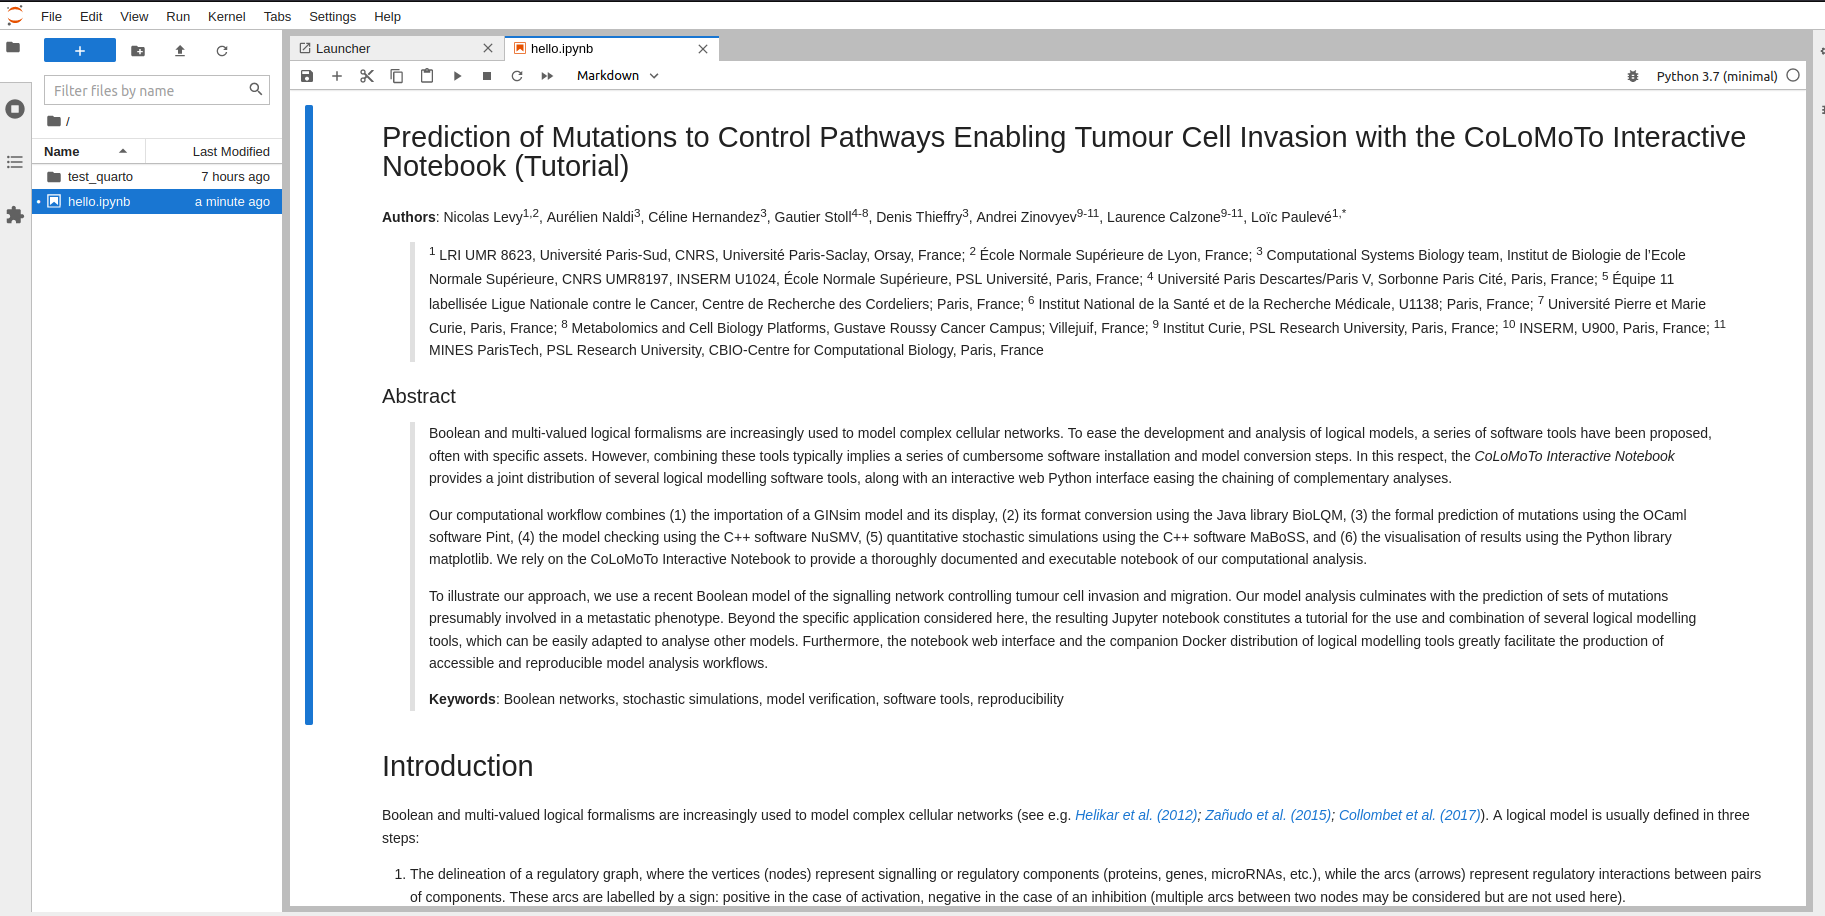
\includegraphics[width=15cm,height=9cm]{images/colomoto_jupyter.png}
\caption{Executable file in Jupyterlab}
\end{figure}}
\only<4>{
\begin{figure}

\includegraphics[width=12cm,height=9cm]{images/colomoto_paper.png}
\caption{Published article}
\end{figure}}
\end{frame}

\subsection*{Markup}
\begin{frame}[<+->]{Markup}
A markup language uses tags to define elements within a document. \newline
Three different types and usage:
\pause
\begin{itemize}
	\item Presentational (used by traditional word-processing systems)
	\item Procedural, provides instructions to process the text (e.g. TeX, PostScript)
	\item Descriptive, to label documents parts (e.g. LaTeX, HTML, XML...)
\end{itemize}
\end{frame}

\begin{frame}{Markdown}
\begin{textblock*}{5cm}(9cm,2cm) % {block width} (coords)

\includegraphics[width=2.3cm,height=1.3cm]{images/Markdown-mark.pdf}
\end{textblock*}
Markdown is a Lightweight markup language
\newline
Designed to be:
\pause
\begin{itemize}[<+->]
	\item easy to write using any generic text editor (plain-text-formatting syntax)
	\item easy to read in the raw format
\end{itemize}
\only<4>{
\begin{textblock*}{10cm}(5cm,4.5cm) % {block width} (coords)
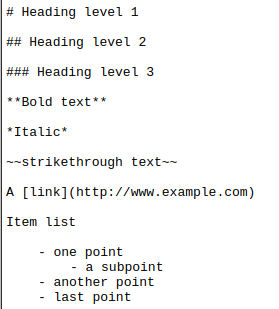
\includegraphics[width=4cm,height=4cm]{images/markdown_syntax.png}
\end{textblock*}}
\onslide<5->{
\vspace{2cm}
Used on Github to make the README.md\\
But how is this useful for literate programming? \\
When you want to weave both code (to be interpreted) and formatting information,\\ you precisely need a lightweight language for the formatting part.}
\end{frame}

\subsection*{Notebooks for bioinformatic}
\begin{frame}
\centering\textbf{R notebooks \emph{vs} Jupyter(Lab) notebook}
\newline

\includegraphics[width=12cm,height=5cm]{images/R-vs-Python.jpg}
\end{frame}

\begin{frame}[<+->]{R notebook}
\begin{enumerate}
	\item Sweave in 2002 \\
\emph{Leisch, Friedrich (2002). ”Sweave, Part I: Mixing R and LaTeX: A short
introduction to the Sweave file format and corresponding R functions”}
	\item knitR in 2011 \\
\emph{”The knitr package was designed to be a transparent engine for dynamic report
generation with R, solve some long-standing problems in Sweave, and combine
features in other add-on packages into one package”}
\end{enumerate}
\end{frame}

\begin{frame}{RMarkdown}
\onslide<1->{
2012 Rmarkdown was born ! \\}
\only<1>{\begin{textblock*}{10cm}(3cm,1.2cm) % {block width} (coords)
\centering
\includegraphics[width=2cm,height=2cm]{images/rmarkdown.png}
\end{textblock*}}
\onslide<2->{
\centering
\includegraphics[width=10cm,height=2cm]{images/rmarkdownflow.png}}
\newline
\onslide<3->{
\emph{”When you run render, R Markdown feeds the .Rmd file to knitr, which executes all of the code chunks and creates a new markdown (.md) document which includes
the code and its output. The markdown file generated by knitR is then processed by pandoc which is responsible for creating the finished format.”}
\footnote{https://rmarkdown.rstudio.com}}
\end{frame}

\begin{frame}{RMarkdown}
\only<1>{\centering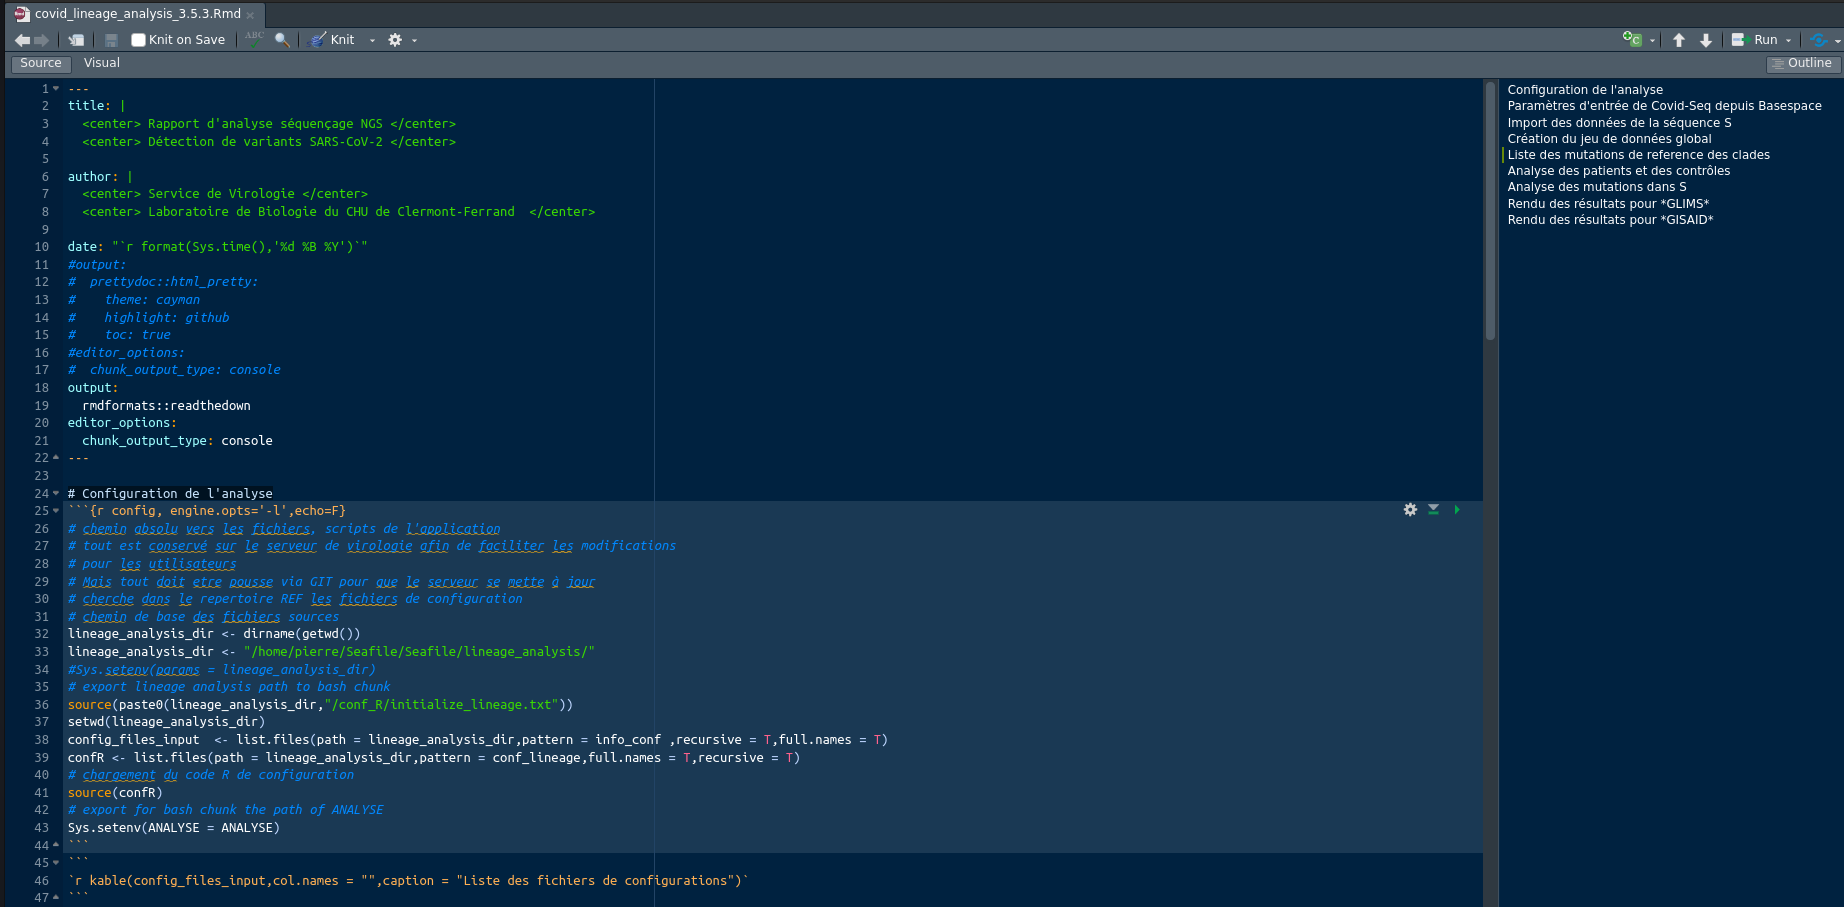
\includegraphics[width=14cm,height=8cm]{images/rmarkdown_example1.png}}
\only<2>{\centering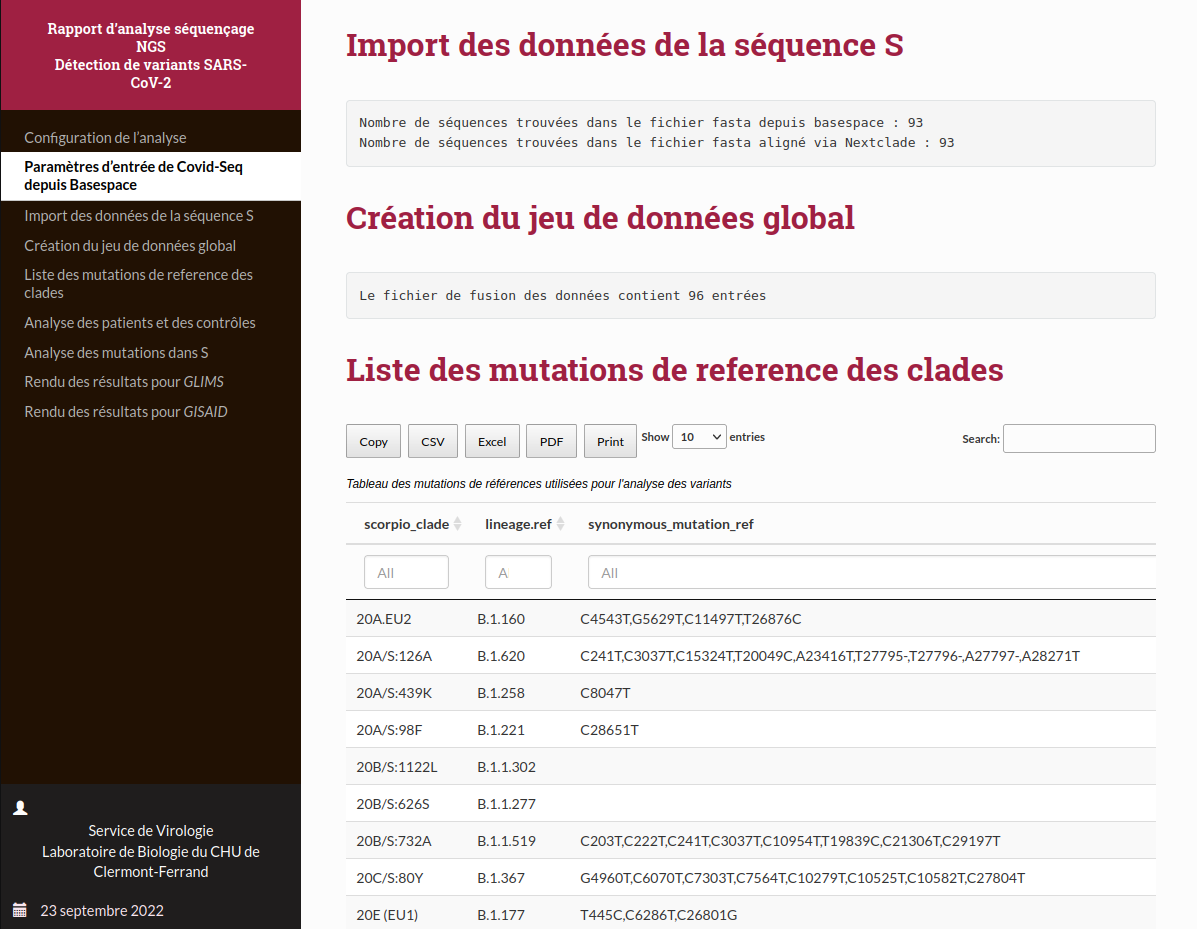
\includegraphics[width=12cm,height=8cm]{images/rmarkdown_example2.png}}
\end{frame}

\begin{frame}[<+->]{Jupyter}
\begin{enumerate}
	\item 2011:  IPython (interactive Python shell) with notebook functionalities
	\item 2014 : Spin-off project called Project Jupyter a non-profit, open-source project maintained by a strong community
		\begin{itemize}
		\item ”Jupyter will always be 100\% open-source software, free for all to use and released under the liberal terms of the modified BSD license”
		\footnote{https://jupyter.org/}
		\item A reference to the three core programming languages supported by Jupyter (Julia, Python and R)
		\end{itemize}
\end{enumerate}
\end{frame}

\begin{frame}{Jupyter}
\onslide<1->{
What is it exactly ?\\
Web-based interactive computational environment}
\begin{itemize}
\item<2-4> Web-based: client/server
\item<3-4> Interactive: notebook system
\item<4-4> Computational environment: console, many kernels available...
\end{itemize}
\onslide<2-4>{\centering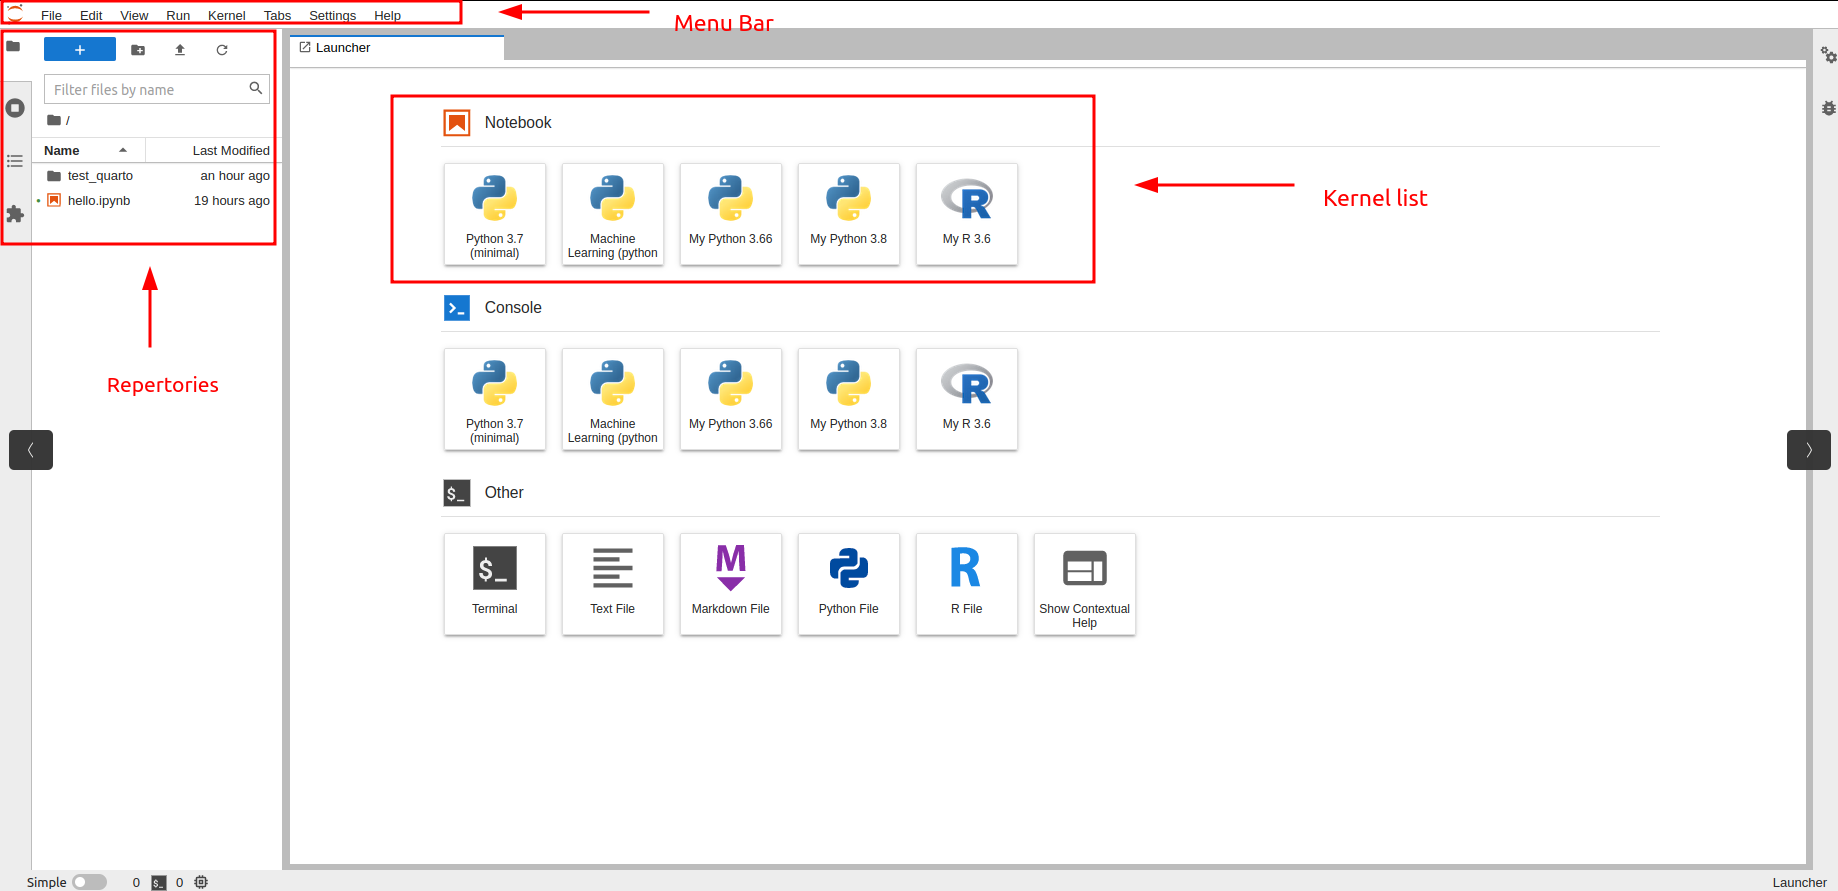
\includegraphics[width=15cm,height=7cm]{images/jupyterlab1.png}}
\only<5>{
\begin{textblock*}{10cm}(1cm,2cm) % {block width} (coords)
\centering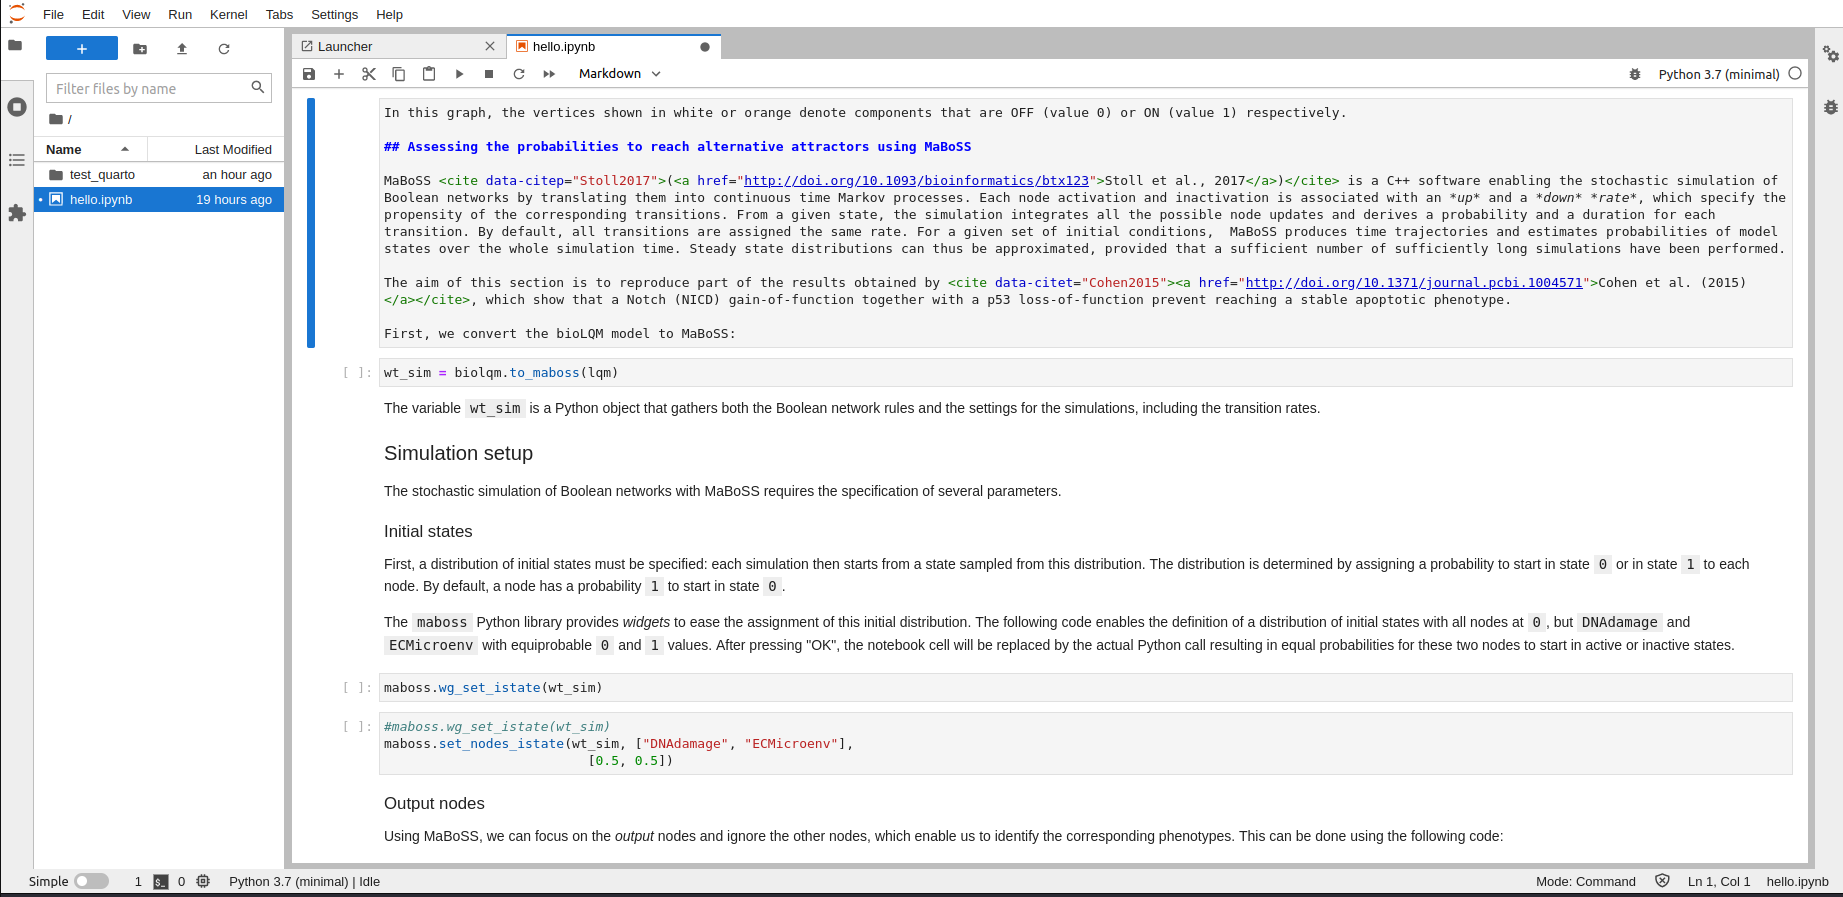
\includegraphics[width=13cm,height=6.5cm]{images/jupyterlab2.png}
\end{textblock*}}
\end{frame}



\section{Practicial training}
\subsection{Build your own documentation}
\begin{frame}

\end{frame}

\end{document}

